\section{Role of Convolution with Pooling}

\subsection{Weight Sharing: Illustrative Example}
\FloatBarrier
\begin{figure}[H]
\centering
\resizebox{\columnwidth}{!}{
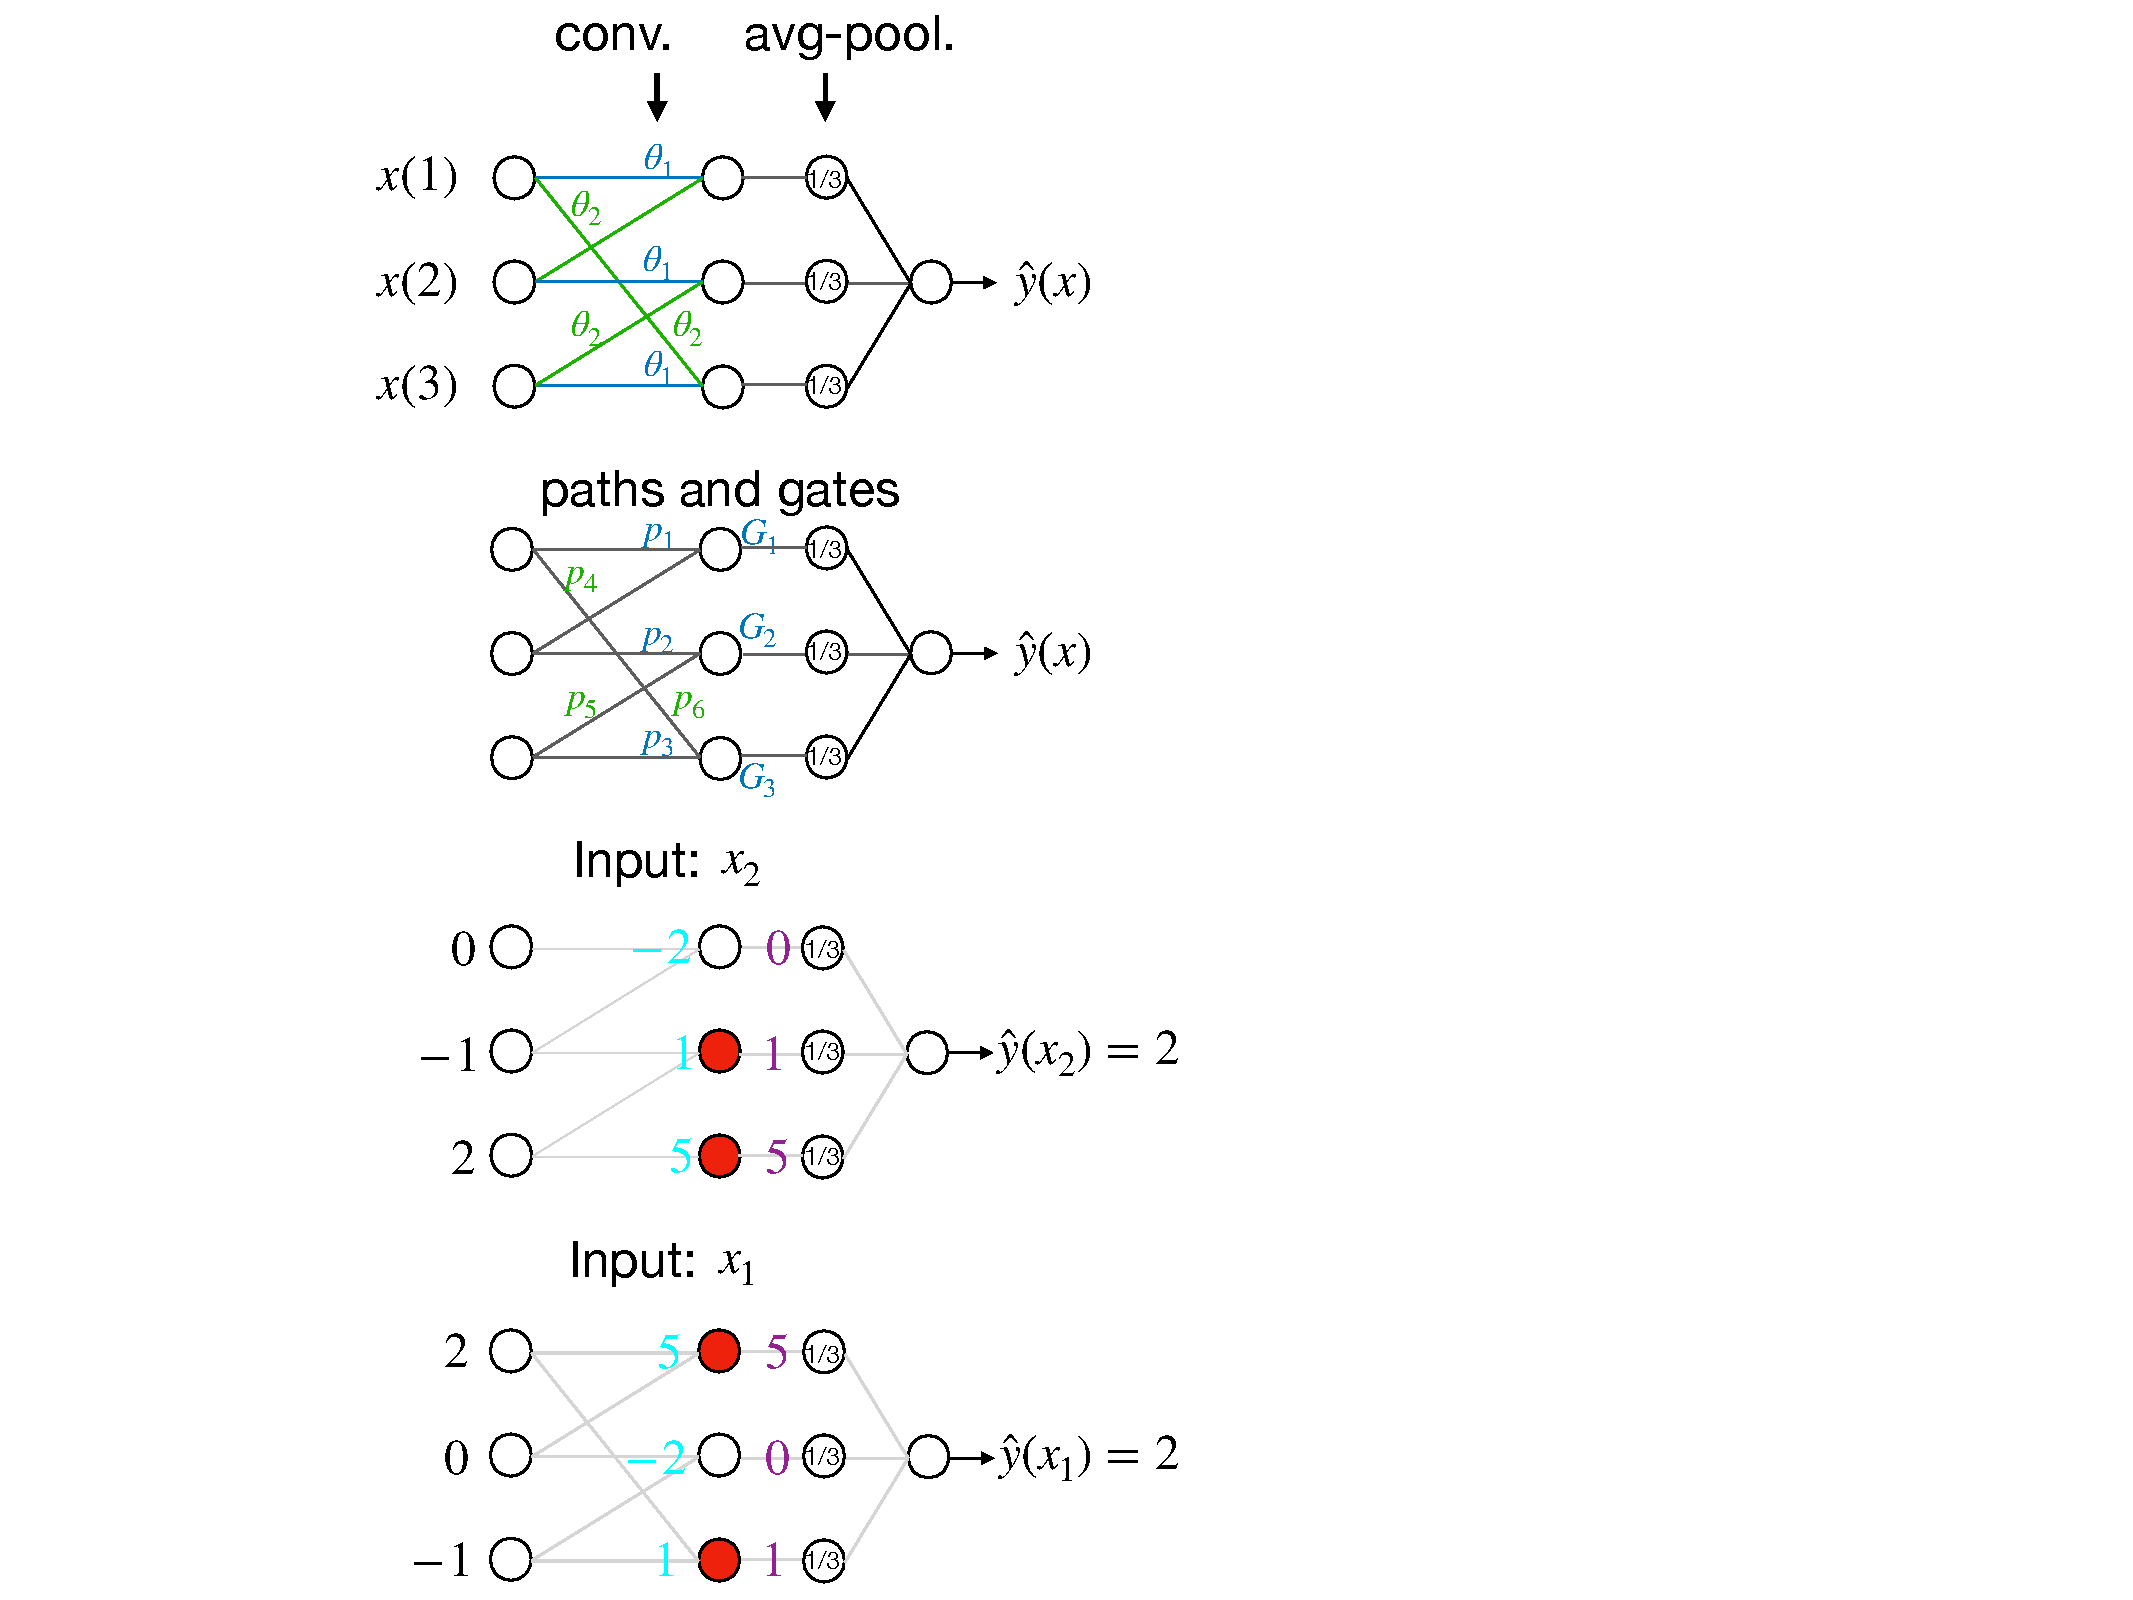
\includegraphics[scale=0.38]{figs/conv.pdf}
}
\end{figure}

\subsection{Circular Convolution With Pooling}

We consider a $1$-dimensional convolutional neural network with circular convolutions (see \Cref{tb:cconv}), with $\dc$ convolutional layers ($l=1,\ldots,\dc$), followed by a \emph{global-average/max-pooling} layer ($l=\dc+1$) and $\dfc$ ($l=\dc+2,\ldots,\dc+\dfc+1$) FC  layers. The convolutional window size is $\wconv<\din$, the number of filters per convolutional layer is $w$, and the width of the FC is also $w$. 
\begin{definition}[Circular Convolution]
For $x\in\R^{\din}$, $i\in[\din]$ and $r\in\{0,\ldots,\din-1\}$, define :

(i) $i\oplus r = i+r$, for $i+r \leq \din$ and $i\oplus r =i+r-\din$, for $i+r>\din$.

(ii) $rot(x,r)(i)=x(i\oplus r), i\in[\din]$.

(iii) $q_{x,\Theta}(\ifout,\iout,l)=\sum_{\icin,\iin}\Theta(\icin,\iin,\iout,l)\cdot z_{x,\Theta}(\ifout\oplus (\icin-1),\iin,l-1)$, where $\iin/\iout$ are the indices (taking values in $[w]$) of the input/output filters. $\icin$ denotes the indices of the convolutional window (taking values in $[\wconv]$) between input and output filters $\iin$ and $\iout$. $\ifout$ denotes the indices (taking values in $[\din]$, the dimension of input features) of individual nodes in a given output filter.
\end{definition}
\begin{definition}[Pooling]
Let $G^{\text{pool}}_{x,\Theta}(\ifout,\iout,\dc+1)$ denote the pooling mask, then we have
\begin{align*}
z_{x,\Theta}(\iout, \dc+1) =\sum_{\ifout} z_{x,\Theta}(\ifout,\iout,\dc)\cdot G^{\text{pool}}_{x,\Theta}(\ifout,\iout,\dc+1),
\end{align*}
where in the case of \emph{global-average-pooling} $G^{\text{pool}}_{x,\Theta}(\ifout,\iout,\dc+1)=\frac{1}{\din},\forall \iout\in[w], \ifout\in[\din]$, and in the case of \emph{$\max$-pooling},  
for a given $\iout\in[w]$, $G^{\text{pool}}_{x,\Theta}(i_{\max},\iout,\dc+1)=1$ where $i_{\max}=\arg\max_{\ifout}z_{x,\Theta}(\ifout,\iout,\dc)$, and $G^{\text{pool}}_{x,\Theta}(\ifout,\iout,\dc+1)=0,\forall \ifout\neq i_{\max}$.
\end{definition}

\begin{proposition}[Rotational Invariance]\label{prop:rot}
Internal variables in the convolutional layers are circularly symmetric,  i.e., for $r\in\{0,\ldots,\din-1\}$ it follows that (i) $z_{rot(x,r),\Theta}(\ifout,\cdot,\cdot) = z_{x,\Theta}(\ifout \oplus r,\cdot,\cdot)$, (ii) $q_{rot(x,r),\Theta}(\ifout,\cdot,\cdot) = q_{x,\Theta}(\ifout \oplus r,\cdot,\cdot)$ and (iii) $G_{rot(x,r),\Theta}(\ifout,\cdot,\cdot) = G_{x,\Theta}(\ifout \oplus r,\cdot,\cdot)$.
\end{proposition}

\subsection{Bundles, Neural Path Feature and Value}
\begin{proposition}
The total number of paths in a CNN is given by  $\Pcnn=\din(\wconv w)^{\dc}w^{(\dfc-1)}$.
\end{proposition}

\begin{notation}[Index Maps]
The ranges of index maps $\Ifeat_l$,  $\Iconv_l$, $\I_l$ are $[\din]$, $[\wconv]$ and $[w]$ respectively. 
\end{notation}

\begin{definition}[Bundle Paths of Sharing Weights]\label{def:bundle}
Let $\hat{P}^{\text{cnn}}=\frac{\Pcnn}{\din}$, and $\{B_1,\ldots, B_{\hat{P}^{\text{cnn}}}\}$ be a collection of sets such that $\forall i,j\in [\hat{P}^{\text{cnn}}], i\neq j$ we have $B_i\cap B_j=\emptyset$ and $\cup_{i=1}^{\hat{P}^{\text{cnn}}}B_i =[\Pcnn]$. Further,  if paths $p,p' \in B_i$, then $\Iconv_l(p)=\Iconv_l(p'), \forall l=1,\ldots, \dc$ and $\I_l(p)=\I_l(p'), \forall l=0,\ldots, \dc$.
\end{definition}

\begin{proposition}\label{prop:bundle}
There are exactly $\din$ paths in a bundle.
\end{proposition}

\begin{definition}\label{def:nps} Let $x\in\R^{\din}$ be the input to the DNN. For this input, 

(i)  $A_{\Theta}(x,p)=\Pi_{l=1}^{\dc+1} G_{x,\Theta}(\Ifeat_l(p),\I_l(p),l)\cdot\Pi_{l=\dc+2}^{\dc+\dfc+1} G_{x,\Theta}(\I_l(p),l)$

(ii)  $\phi_{x,\Theta}(\hat{p})\eqdef \sum_{\hat{p}\in B_{\hat{p}}}x(\Ifeat_0(p))A_{\Theta}(x,p)$.

(iii)  $v_{\Theta}(B_{\hat{p}})\eqdef \Pi_{l=1}^{\dc} \Theta(\Iconv_{l}(p),\I_{l-1}(p),\I_{l}(p),l) \cdot \Pi_{l=\dc+2}^{\dc+\dfc+1} \Theta(\I_{l-1}(p),\I_l(p),l)$, for any $p\in B_{\hat{p}}$.

The NPF is defined as $\phi_{x,\Theta}\eqdef (\phi_{x,\Theta}(B_{\hat{p}}),\hat{p}\in [\hat{P}^{\text{cnn}}])\in\R^{\hat{P}^{\text{cnn}}}$. The NPV is defined as $v_{\Theta}\eqdef (v_{\Theta}(B_{\hat{p}}),\hat{p}\in [\hat{P}^{\text{cnn}}])\in\R^{\hat{P}^{\text{cnn}}}$.
\end{definition}

\subsection{Neural Path Kernel}
\begin{definition}\label{def:cnnlambda}
Define $\Lambda_{\Theta}(i,x,x_{s'}) \eqdef \left|\{p\in[P]\colon  \I_0(p)=i, A_{\Theta}(x_s,p)= A_{\Theta}(x_{s'},p)=1\}\right|$ to be total number of `active' paths for both $x_s$ and $x_{s'}$ that pass through input node $i$.
\end{definition}

\begin{lemma}[Rotational Invariant Kernel]\label{lm:cnnnpk}
Let $H^{\text{cnv}}_{\Theta}$ denote the NPK of a CNN, then 
\begin{align*}
H^{\text{cnv}}_{\Theta}(s,s')=\sum_{r=0}^{\din-1} \ip{x_s,rot(x_{s'},r)}_{\Lambda(\cdot, x_s,rot(x_{s'},r))}=\sum_{r=0}^{\din-1} \ip{rot(x_s,r),x_{s'}}_{\Lambda(\cdot, rot(x_s,r),x_{s'})}
\end{align*}
\end{lemma}


